\documentclass[11pt,a4paper]{scrartcl}
 \usepackage[backend=bibtex,style=numeric, sorting=none,defernums=true]{biblatex}
\bibliography{references}
\DeclareBibliographyCategory{pat}
\DeclareBibliographyCategory{groupA}
\DeclareBibliographyCategory{groupB}
\defbibheading{empty}

%In case we want to use a sans serif font (see 54_012)
\usepackage{helvet}
%\renewcommand{\familydefault}{\sfdefault}

\usepackage{anysize} \marginsize{18mm}{18mm}{2mm}{7mm} % Right, left, top, bottom
\usepackage{graphicx}
\usepackage{wrapfig}
\usepackage{color}
\usepackage[table]{xcolor}
\newcommand{\tabitem}{-~~}%{\textbullet}
\usepackage{calc, fp}
\usepackage[group-separator={,}]{siunitx}
\sisetup{detect-weight=true, detect-family=true}
\usepackage{tabularx}
\usepackage{tikz}
\usetikzlibrary{positioning}
\usepackage{float}
\usepackage{units}
\usepackage{ifpdf}
\usepackage[caption=false,font=footnotesize]{subfig}
\usepackage{afterpage}
\usepackage{multirow}
\usepackage{eurosym}
\usepackage{todonotes} 
\usepackage{gensymb}

\newcommand{\GroupAlg}{Institute of Science}
\newcommand{\GroupA}{IoS}
\newcommand{\GroupAUniversity}{Universit\"at Hamburg} 
\newcommand{\GroupAProf}{Prof.\ Science}
\newcommand{\GroupAEmployment}{Full Professor (W3)}

\newcommand{\GroupBlg}{Institute of Research}
\newcommand{\GroupB}{IoR}
\newcommand{\GroupBUniversity}{Universit\"at München} 
\newcommand{\GroupBProf}{Prof.\ Research}
\newcommand{\GroupBEmployment}{Full Professor (W2)}

\newcommand{\proposalTitle}{Reasearch Proposal}

\newcommand\Fig[1]{{Fig}.~\ref{#1}}
\newcommand\fig[1]{{Fig}.~\ref{#1}}
\newcommand\Tab[1]{{Tab}.~\ref{#1}}
\newcommand\tab[1]{{tab}.~\ref{#1}}
\newcommand\Equ[1]{{Eq}.~(\ref{#1})}
\newcommand\equ[1]{{eq}.~(\ref{#1})}

\long\def\desc#1{}

\def\WPDesc[#1]#2#3#4#5#6{\vspace{5mm} \hspace{-2mm}  \begin{tabular}{p{1.4cm}|p{2.5cm}|p{12.2cm}|} \hline \rowcolor[gray]{0.9}
		\multicolumn{1}{|l}{\textbf{#1}} & \multicolumn{2}{|l|}{\textbf{ #2 }} \\
		\hline
		& Partners [pm]   & #3 \\
		\cline{2-3}  & Dependencies    & #4 \\
		\cline{2-3}  & Results, Tasks  & #6 \\
		\cline{2-3}  & Start - End     & #5 \\
		\cline{2-3}
	\end{tabular}
}

\newcommand{\WPDescStyle}[6]{
	\vspace{4pt}
	\noindent
	\begin{tabular}{p{2.4cm}|p{4.4cm}p{2.4cm}|p{6.5cm}} %{p{2.4cm}|p{14.2cm}} 
		\multicolumn{1}{l}{\textit{#1}} & \multicolumn{3}{l}{\textit{#2}} \\
		\hline
		\cellcolor[gray]{0.9}Partners [pm]   &\cellcolor[gray]{0.9}\small #3 & \cellcolor[gray]{0.9} & \cellcolor[gray]{0.9} \small #5\\
		
		\cellcolor[gray]{0.9}Dependencies    & \cellcolor[gray]{0.9}\small #4 &\cellcolor[gray]{0.9}&\cellcolor[gray]{0.9} \\
		%\cellcolor[gray]{0.9}Dependencies    & \multicolumn{3}{l}{\cellcolor[gray]{0.9}\small #4} \\
		\hline
		%\cellcolor[gray]{0.9} Results  &  \multicolumn{3}{p{14.2cm}}{\cellcolor[gray]{0.9} {\raggedright \small #6}} \\ %\hline
%		Start - End     & \small #5 \\                \hline
	\end{tabular}
	\vspace{2.6pt}
}

\begin{document}
\newcommand{\HRule}{\rule{\linewidth}{1pt}}

\begin{center}
  {\noindent\fontfamily{\sfdefault}\LARGE\bfseries\proposalTitle } \\[18pt]
\end{center}

\noindent\begin{minipage}{0.43\textwidth}
	\begin{center} 
		\fontfamily{\sfdefault}
		%		\large
		\textbf{\GroupAProf} \\[6pt]% Your name
		\emph{\GroupA}\\[1pt]
		\textsf{\GroupAUniversity\\[6pt]
		\GroupAEmployment\\permanent employment}
	\end{center}
 \end{minipage}
\hfill
\noindent\begin{minipage}{0.43\textwidth}
	\begin{center} 
		\fontfamily{\sfdefault}
		%		\large
		\textbf{\GroupBProf} \\[6pt]% Your name
		\emph{\GroupB}\\[1pt]
		\textsf{\GroupBUniversity\\[6pt]
		\GroupBEmployment\\permanent employment}
	\end{center}
 \end{minipage}





\setcounter{page}{1}
\vspace{6pt}

\section{State of the art and preliminary work} \label{sec:stateOfTheArt}

Discuss state-of-the-art and cite some work \cite{976921}.
\subsection*{Preliminary work}

The preliminary work of your group and others on the topic.

\subsection{Project-related publications}

\subsubsection*{Peer-reviewed articles, books, and journals}

\defbibenvironment{bibliography}
{\list
	{\printtext[labelnumberwidth]{%
			\printfield{prefixnumber}%
			\printfield{labelnumber}}}
	{\setlength{\labelwidth}{\labelnumberwidth}%
		\setlength{\leftmargin}{\labelwidth}%
		\setlength{\labelsep}{\biblabelsep}%
		%      \addtolength{\leftmargin}{\labelsep}%
		\addtolength{\leftmargin}{6pt}% <-- changed
		\setlength{\itemsep}{\bibitemsep}%
		\setlength{\parsep}{\bibparsep}}%
	\renewcommand*{\makelabel}[1]{\hss##1}}
{\endlist}
{\item}

\setlength{\bibitemsep}{0pt}
\setlength{\bibhang}{0pt}

\addtocategory{groupA}{JOSEPH201736}
\addtocategory{groupB}{7961256}
\addtocategory{pat}{e2009circuits}


\nocite{JOSEPH201736, 7961256, e2009circuits}

\renewcommand*{\bibfont}{\footnotesize}

\printbibliography[category=groupA,heading=empty]
\vspace{-\baselineskip}
\printbibliography[category=groupB,heading=empty] %,maxbibnames=2]



\subsubsection*{Patents}
\printbibliography[category=pat,heading=empty]




\section{Objectives and work program}
\label{sec:objectives_and_work_programme}

\subsection{Anticipated total duration of the project}
\label{sec:anticipated_total_duration_of_the_project}
The application period is 36 months; the support is requested for the whole 36 months. 
The favored starting date of funding is August 1st, 2019 or shortly after approval.


\subsection{Objectives}
\label{sec:objectives}

Introduce your objectives. Don't forget your research hypothesis.

\subsubsection{Outcomes}

This section is just a suggestion, I usually like it a lot. Not required by standards.

\subsubsection{Limitations of today's approach}

This section is just a suggestion, I usually like it a lot. Not required by standards.

\subsubsection{Potential for optimization} \label{sec:objectives:motivation}

This section is just a suggestion, I usually like it a lot. Not required by standards.
\subsection{Work program incl. proposed research methods}

Maybe give a short introduction.
\begin{figure}[t]
        \centering
	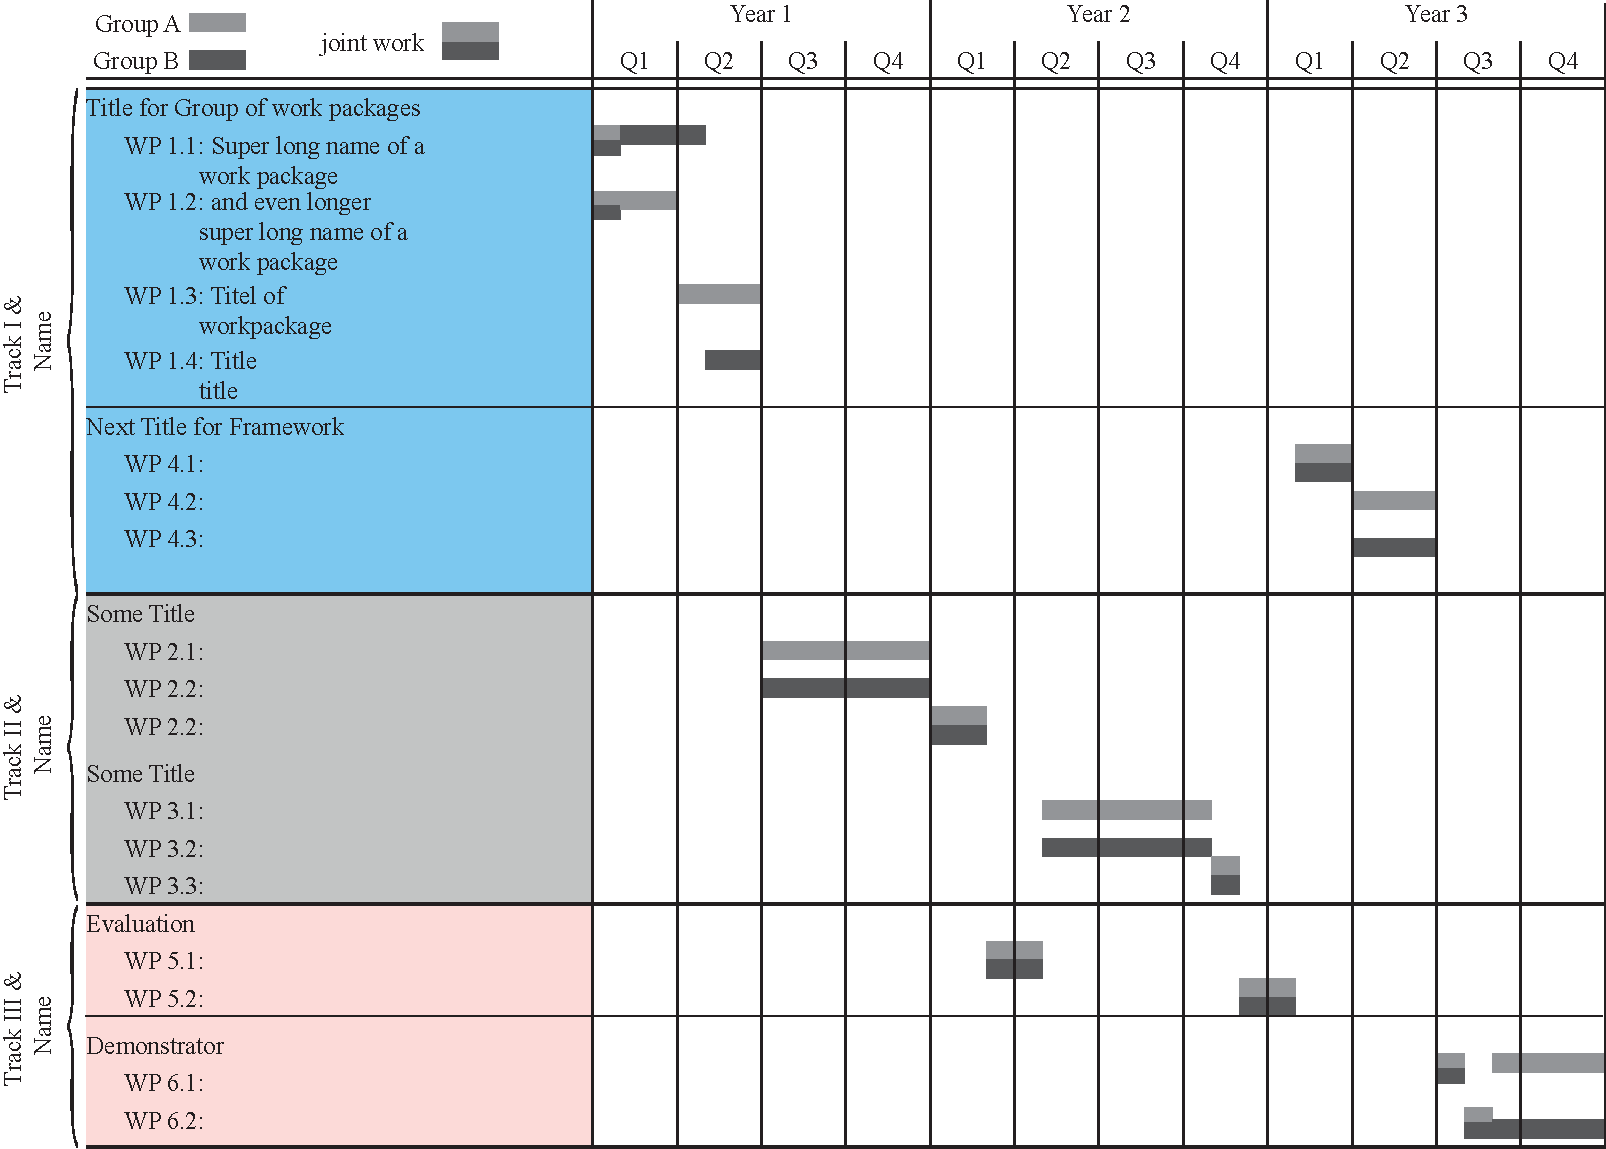
\includegraphics[width=\columnwidth]{figures/workplan}
	\caption{\vspace{-2pt}Project structure}
	\label{fig:project_structure}
	\vspace{-10pt}
\end{figure}


\subsubsection{Work Packages}

\subsubsection*{WP 1: Simulation and Exploration Framework (Track: Methodologies and Tools)} 

\WPDescStyle{WP 1.1}{Title of this work package}{\GroupA~[3.5], \GroupB~[0.5]}{WP 1.1}{From M1 to M4}{
 \tabitem xxx \newline
 \tabitem xxx
}

\noindent some description.



\WPDescStyle{WP 1.2}{Title of this work package}{\GroupB~[3.5], \GroupA~[0.5]}{WP 1.1}{From M1 to M4}{
	\tabitem xxx \newline
	\tabitem xxx
}

\noindent some description.





\subsection{Data handling}
No special measures are required beside the usual DFG guidelines for good scientific practice.

\subsection{Other information}
Not applicable.

\vspace{-2mm}
\subsection{Descriptions of proposed investigations involving experiments on humans, human materials or animals}
%\subsection{Explanations on the proposed investigations}
Not applicable.

\vspace{-2mm}
\subsection{Information on scientific and financial involvement of international cooperation partners}
Not applicable.

\vspace{-2mm}
\section{Bibliography}

\begingroup
\renewcommand*{\bibfont}{\footnotesize}
%\setstretch{0.8}
\setlength\bibitemsep{0pt}
\sloppy
\printbibliography[heading=empty,notcategory=groupA,notcategory=groupB, notcategory=pat] %,maxbibnames=3
\endgroup

\vspace{-2mm}
\FPset \Months{36}
\FPset \Years{3}

\FPset \GroupAbaSalery{472.40} 
\FPset \GroupAmaSalery{472.40} 
\FPset \GroupBbaSalery{505.56} 
\FPset \GroupBmaSalery{687.72} 

\FPset \wiMASalery{66400} %http://www.dfg.de/formulare/60_12/60_12_de.pdf

\FPmul \itemWiMASalery \Years \wiMASalery
\FPmul \iiktWiMASalery \Years \wiMASalery
\FPadd \totalWiMASalery \itemWiMASalery \iiktWiMASalery
\FPround \itemWiMASalery \itemWiMASalery {0}
\FPround \iiktWiMASalery \iiktWiMASalery {0}
\FPround \totalWiMASalery \totalWiMASalery {0}

\FPmul \GroupAbaSaleryTotal \Months \GroupAbaSalery
\FPmul \GroupAmaSaleryTotal \Months \GroupAmaSalery
\FPmul \GroupBbaSaleryTotal \Months \GroupBbaSalery
\FPmul \GroupBmaSaleryTotal \Months \GroupBmaSalery

\FPadd \HiWiTotalSalery {0} \GroupAbaSaleryTotal
\FPadd \HiWiTotalSalery \HiWiTotalSalery \GroupAmaSaleryTotal
\FPadd \HiWiTotalSalery \HiWiTotalSalery \GroupBmaSaleryTotal

\FPadd \HiWiGroupATotalSalery \GroupAbaSaleryTotal \GroupAmaSaleryTotal
\FPadd \HiWiGroupBTotalSalery \GroupBbaSaleryTotal \GroupBmaSaleryTotal

\FPround \HiWiGroupATotalSalery \HiWiGroupATotalSalery {2}
\FPround \HiWiGroupBTotalSalery \HiWiGroupBTotalSalery {2}

\FPround \HiWiTotalSalery \HiWiTotalSalery {2}

\FPround \GroupAbaSaleryTotal \GroupAbaSaleryTotal {2}
\FPround \GroupAmaSaleryTotal \GroupAmaSaleryTotal {2}
\FPround \GroupBbaSaleryTotal \GroupBbaSaleryTotal {2}
\FPround \GroupBmaSaleryTotal \GroupBmaSaleryTotal {2}

\FPadd \totalSalery \HiWiTotalSalery \totalWiMASalery
\FPround \totalSalery \totalSalery {0}




\section{Requested modules/funds}
We are applying for the "Basic Module" in the research grants programme. 

\subsection{Funding for staff}
\subsubsection{Research staff}

\paragraph{Postdoctoral researcher or comparable}

\noindent Not applicable.

\paragraph{Doctoral researcher or comparable}

\noindent We apply for \textbf{a total amount of \euro \num[group-separator={,}]{\totalSalery}}.

For \GroupAProf\ (\GroupAlg--\GroupA) and \GroupBProf\ (\GroupBlg--\GroupB) we
apply for \euro \num[group-separator={,}]{\itemWiMASalery} each for \Months months of funding for one doctoral
researcher. The researchers will work 100\% of the standard work week
on the project and conduct the research. Employing a researcher in
wage group TVL E-13 for one year costs \euro \num[group-separator={,}]{\totalWiMASalery}.

\vspace{6pt}
\noindent\begin{tabular}{lrrrr}
\bfseries Position && \bfseries Amount &\bfseries Factor &\bfseries Subtotal \\\hline
Doctoral researcher at \GroupA & TVL E-13 per year & \euro \num[group-separator={,}]{\wiMASalery} & \Years & \euro \num[group-separator={,}]{\itemWiMASalery}\\
Doctoral researcher at \GroupB & TVL E-13 per year & \euro \num[group-separator={,}]{\wiMASalery} & \Years & \euro \num[group-separator={,}]{\iiktWiMASalery}
\\\cline{5-5}
\bfseries Total & && &  \bfseries \euro \num[group-separator={,}]{\totalWiMASalery}\\
\end{tabular}
\vspace{6pt}

\paragraph{Other research assistant}

\noindent Not applicable.

\subsubsection{Non-academic staff member}

\noindent Not applicable.

\subsubsection{Miscellaneous staff}

\paragraph{Support staff (research support staff and student assistants)}


\noindent We apply for a {\bfseries total amount of \euro \num[group-separator={,}]{\HiWiTotalSalery}} for support staff.


For \GroupAProf~(\GroupA) we apply for funding of two student assistants to support the academic staff with implementation, simulation, and evaluation with the amount of \euro \num[group-separator={,}]{\HiWiGroupATotalSalery}. Each assistant will work 40 hours per month during the duration of the project. The pre-tax wage at \GroupA\ is \euro \num[group-separator={,}]{\GroupAbaSalery} independent of the students degree. 

For \GroupBProf~(\GroupB) we also apply for funding of two student assistants with the amount of \euro \num[group-separator={,}]{\HiWiGroupBTotalSalery}. The pre-tax wage at \GroupB\ is \euro \num[group-separator={,}]{\GroupBbaSalery} for bachelor students per month and \euro \num[group-separator={,}]{\GroupBmaSalery} a for master student.

\vspace{6pt}
\noindent\begin{tabular}{lrrr}
\bfseries Position & \bfseries Amount &\bfseries Factor &\bfseries Subtotal \\\hline
Bachelor student at \GroupA, 40 hours & \euro \GroupAbaSalery & \Months & \euro \num[group-separator={,}]{\GroupAbaSaleryTotal}\\
Master student at \GroupA, 40 hours & \euro \GroupAmaSalery & \Months & \euro \num[group-separator={,}]{\GroupAmaSaleryTotal}\\
Bachelor student at \GroupB, 40 hours & \euro \GroupBbaSalery & \Months & \euro\num[group-separator={,}]{\GroupBbaSaleryTotal}\\
Master student at \GroupB, 40 hours & \euro \GroupBmaSalery & \Months & \euro \num[group-separator={,}]{\GroupBmaSaleryTotal}\\
\bfseries Total & & &  \bfseries \euro \num[group-separator={,}]{\HiWiTotalSalery}\\
\end{tabular}
\vspace{6pt}

\paragraph{Other staff}
\noindent Not applicable.

\subsection{Funding for direct project costs}
\subsubsection{Equipment up to \euro10,000, software and consumables}

\noindent We apply for a {\bfseries total amount of \euro 16,500} for equipment. 

We apply for the amount of \euro 5,500 for each of the groups
(\GroupAProf and \GroupBProf ) for a "Xilinx
Virtex UltraScale FPGA VCU108 Evaluation Kit".  An state-of-the-art
FPGA board is required for prototyping. After finishing this project the
prototyping boards can also be used for other research activities.

\subsubsection{Travel}

\noindent We apply for a {\bfseries total amount of \euro 20,000} for travel expenses. 

We apply for funding of the expenses for conference travels to the amount of \euro 8,000 for \GroupAProf~(\GroupA) for two European and two International conferences; we apply for funding of the expenses for conference travels to the amount of \euro 8,000 for \GroupBProf~(\GroupB) for two European and two International conferences:

\vspace{6pt}
\noindent\begin{tabular}{lrrr}
\bfseries Position & \bfseries Amount &\bfseries Factor &\bfseries Subtotal \\\hline
European conference (\GroupA) & \euro 1,500 & 2 & \euro 3,000\\
International conference (\GroupA) & \euro 2,500 & 2 & \euro 5,000\\
European conference (\GroupB) & \euro 1,500 & 2 & \euro 3,000\\
International conference (\GroupB) & \euro 2,500 & 2 & \euro 5,000\\   
\bfseries Total & & &  \bfseries \euro 20,000\\
\end{tabular}
\vspace{6pt}

\noindent In addition, for cooperation within this project we apply
for \euro 4,210 for \GroupAProf\ (\GroupA) , \euro 4,210 for
\GroupBProf~(\GroupB). There are five
joined work packages (WP 5.1, WP 5.2, WP 5.3, WP 7.3, WP 7.4) and five
work packages requiring close cooperation (WP 1.3, WP 2.3, WP 3, WP 4,
WP 7.2). Therefore we ask for the travel expenses for 10 meetings, in
which two persons are visiting the project partner.
We assume a duration of half a work week per meeting (2 nights). Thus,
per person and trip two railway tickets, two nights at a hotel, and
three daily allowances are required, which amounts to:

\vspace{6pt}
\noindent\begin{tabular}{lrrr}
\bfseries Position & \bfseries Amount &\bfseries Factor &\bfseries Subtotal \\\hline
Railway ticket, single trip per person & \euro 65.00 & 40=10*2*2 & \euro 2,600\\
Accommodation per night and person & \euro 80.00 & 40=10*2*2 & \euro 3,200\\
Daily allowance & \euro 24.00 & 60=10*3*2 & \euro 1,440 \\\cline{4-4}
\bfseries Total & & &  \bfseries \euro 8,240\\
\end{tabular}
\vspace{6pt}


\subsubsection{Visiting researchers}

\noindent Not applicable.

\subsubsection{Experimental animals}

\noindent Not applicable.

\subsubsection{Other}

\noindent Not applicable.

\subsubsection{Project-related publication expenses}
\noindent At least four open-access journal publications are expected. This requires additional fees for handling
and open access services of about 1,500 EUR. Our universities employ
an open access strategy already. However, researchers are encouraged
to acquire additional funding for open access publishing. Therefore We
apply for a {\bfseries total amount of \euro 1,500} to pay fees of
journal publications. For \GroupAProf~(\GroupA) we apply for \euro 750 and
for \GroupBProf~(\GroupB) we apply for \euro 750 as well.

\subsection{Funding for instrumentation}

\noindent Not applicable.



\section{Project requirements}
\subsection{Employment status information}

\begin{itemize}\setlength{\itemsep}{0pt}
	\item {\bfseries \GroupAProf}, \GroupAlg, \GroupAUniversity,  \GroupBEmployment, permanent employment
	\item {\bfseries \GroupBProf}, \GroupBlg, \GroupBUniversity,  \GroupAEmployment, permanent employment
\end{itemize}

\subsection{First-time proposal data}
Not applicable.


\subsection{Composition of the project group}

\begin{itemize}\setlength{\itemsep}{0pt}
	\item {\bfseries \GroupAProf}, \GroupAlg, \GroupAUniversity,  \GroupBEmployment, permanent employment
	\item {\bfseries \GroupBProf}, \GroupBlg, \GroupBUniversity,  \GroupAEmployment, permanent employment
\end{itemize}


\subsection{Cooperation with other researchers}

\subsubsection{Researchers with whom you have agreed to cooperate on this project}
Not applicable.

\subsubsection{Researchers with whom you have collaborated scientifically within the past three years}

\small

\begin{itemize}\setlength{\itemsep}{0pt}
\item {\bfseries Prof.\ Awesome}, The University of York (UK) 
\item {\bfseries Prof.\ Cool}, Some other University
\end{itemize}

\subsection{Scientific equipment}

\noindent The following equipment is available at the \textit{\GroupA} during the project:
\vspace{-6pt}
 
\begin{itemize}\setlength{\itemsep}{0pt}
\item Some stuff
\item even more stuff
\end{itemize}

\vspace{-6pt}
\noindent The following equipment is available at the \textit{\GroupB} during the project:
\vspace{-6pt}

\begin{itemize}\setlength{\itemsep}{0pt}
\item Some stuff
\item even more stuff
\end{itemize}


\subsection{Project-relevant interests in commercial enterprises}
Not applicable.

\subsection{Project-relevant participation in commercial enterprises}
Not applicable.

\section{Additional information}
Not applicable.

\end{document}